\documentclass{article}
\usepackage{tikz}
\usetikzlibrary{arrows.meta}

\begin{document}

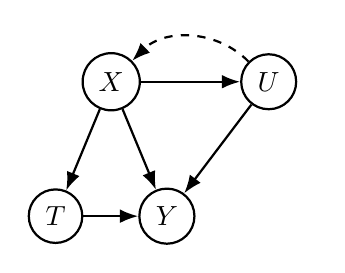
\begin{tikzpicture}[node distance=1cm, thick, main/.style={circle, draw, minimum size=0.5cm}]
    \node[main] (X) {$X$};
    \node[main] (U) [right of=X, xshift=1cm] {$U$};
    \node[main] (T) [below left of=X, yshift=-1cm] {$T$};
    \node[main] (Y) [below right of=X, yshift=-1cm] {$Y$};

    \draw[-Latex] (X) -- (U);
    \draw[-Latex] (X) -- (T);
    \draw[-Latex] (X) -- (Y);
    \draw[-Latex] (U) -- (Y);
    \draw[-Latex] (T) -- (Y);
    
    \draw[dashed, -Latex] (U) to[bend right=45] (X);
    
    \node[] at (2.5,-1.5) {};
\end{tikzpicture}

Example causal graph with hidden confounding. $X$: Observed covariates, $U$: Hidden confounders, $T$: Treatment, $Y$: Outcome. Direct edges denote causal relations and the bidirectional edge signifies possible correlation.
\end{document}